\documentclass{article}

% set font encoding for PDFLaTeX, XeLaTeX, or LuaTeX
\usepackage{ifxetex,ifluatex}
\if\ifxetex T\else\ifluatex T\else F\fi\fi T%
  \usepackage{fontspec}
\else
  \usepackage[T1]{fontenc}
  \usepackage[utf8]{inputenc}
  \usepackage{lmodern}
\fi

\usepackage{hyperref, amssymb, amsmath, multicol, graphicx, paracol}

\usepackage[margin=0.8in]{geometry}

\pagenumbering{gobble}


\newcommand{\R}{\mathbb{R}}


\begin{document}


\begin{center}
\begin{Huge}Limits and Continuity Exercises\end{Huge}
\end{center}


\subsection*{A. Are the following true or false? If true, explain why. If false, give a counter-example.}
\begin{enumerate}
\item If $\displaystyle\lim_{x\to a} f(x)$ does not exist, then $f$ is undefined at the point $x=a$.
\item If a function is not defined at $x=a$, then $\displaystyle\lim_{x\to a} f(x)$ does not exist.
\item If $f$ and $g$ are continuous on their domains which contain $a$, then $\displaystyle\lim_{x\to a} f(x) + g(x) = f(a) + g(a).$
\item If $\displaystyle\lim_{x\to a} f(x)$ exists, then $f$ is continuous at $a$.
\end{enumerate}


\subsection*{B. Evaluate the following limits (or say that the limit DNE):}

\begin{multicols}{4}

\begin{enumerate}
\item $\displaystyle\lim_{x\to 3}\frac{x^2-9}{x+3}$
\item $\displaystyle\lim_{x\to 3}\frac{x^2-9}{x-3}$
\item $\displaystyle\lim_{x\to \pi/2}\frac{\cot(x)}{\cos(x)}$
\item $\displaystyle\lim_{x\to 6}\frac{10}{x^2-36}$
\item $\displaystyle\lim_{x\to \infty}\tan(x)$
\item $\displaystyle\lim_{x\to\pi/2^+} \tan(x)$
\item $\displaystyle\lim_{x\to \infty}\frac{x^3+3x^2+4}{1-x^2}$
\item $\displaystyle\lim_{x\to \infty}\frac{\cos(x)}{x^2}$
\item $\displaystyle\lim_{x\to \infty}\frac{4x^4+3x^3}{7x^4+x}$
\item $\displaystyle\lim_{x\to \infty}\frac{10000x^3-x^2}{8x^4+2x+1}$
\item $\displaystyle\lim_{x \rightarrow 1^+} \frac{x^2+x+1}{x^2-1}$
\item $\displaystyle\lim_{x\to 0}\frac{(\cos^2(x) - 1)(x+3)}{x}$
\item $\displaystyle\lim_{x\to 5}x^3+e^x\sin(x)$
\item $\displaystyle\lim_{x\to 5}\frac{6\sin(x-5)}{x-5}$
\end{enumerate}

\end{multicols}

\subsection*{C. For each function $f$, find a value of $c$ so that $f$ is continuous on $\mathbb{R}$:}
\begin{multicols}{2}
\begin{enumerate}
\item $f(x)=\begin{cases}2x & x \leq c \\ x^2+1 & x > c.\end{cases}$
\item $f(x)=\begin{cases}2x+c & x < 2 \\ x^2 + cx +1 & x \geq 2.\end{cases}$
\end{enumerate}
\end{multicols}

\subsection*{D. Answer the following questions based on the graph (each box has width 1).}
\columnratio{0.4}
\begin{paracol}{2}
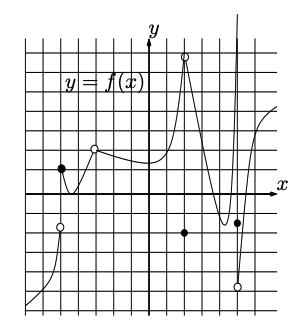
\includegraphics[width=2in]{img/piecewise.png}
\switchcolumn
\vspace{2em}

\begin{enumerate}
\item At what points $a$ does $\displaystyle \lim_{x\to a} f(x)=L$ but $L\neq f(a)$?
\item At which points is $f$ not continuous?
\item Does $\displaystyle\lim _{x \to 2^{-}} f(x)$ exist? If it does, what is its value?
\item Does $\displaystyle\lim _{x \to 2^{+}} f(x)$ exist? If it does, what is its value?
\item Does $\displaystyle\lim _{x \to 2} f(x)$ exist? If it does, what is its value?
\item What is $f(2)$?
\end{enumerate}
\end{paracol}


\subsection*{E. Answer the following questions based on the function $f$ defined below.}
% \columnratio{0.4}
\begin{multicols}{2}
$$f(t)=\begin{cases}
1+t & t<0 \\
t^2+1 & 0 \leq t<1 \\ 
3 & t=1 \\
t+4 & t>1
\end{cases}$$
\columnbreak
% \switchcolumn
\begin{enumerate}
\item What is $\displaystyle\lim_{t\to 0}f(t)$?
\item What is $\displaystyle\lim_{t\to 0^+}f(t)$?
\item What is $\displaystyle\lim_{t\to 0^-}f(t)$?
\item Where is $f$ continuous?
\end{enumerate}
\end{multicols}


\newpage

\subsection*{Answers (in no particular order)}

\begin{itemize}

\item $-5$, $-3$, $2$, $5$
\item 0
\item 6
\item $-1$
\item False ($f(x)=\frac{x^2}{x}$ is not defined at 0, but $\lim_{x\to 0}f(x) = 0$)
\item 1
\item 6
\item 1
\item $-3$, $2$
\item DNE
\item False ($f(x)=\frac{|x|}{x}$ is not continuous at 0, but $\lim_{x\to 0}f(x) = 0$)
\item $-\infty$
\item 1
\item $125+e^5\sin(5)$
\item DNE
\item $\infty$
\item -2
\item True (Since $f$ and $g$ are continuous, so is $f+g$. Then by the def. of continuity, $\displaystyle\lim_{x\to a} f(x)+g(x)=f(a) + g(a)$)
\item 0
\item $(\infty,1)\cup(1,\infty)$
\item False (If $f(x)=\begin{cases}1 & x\geq 0 \\ -1 & x < 0\end{cases}$ then $\displaystyle\lim_{x\to a} f(x)$ but $f(0)=1$)
\item 1
\item yes, $6.8$
\item $0$
\item yes, $6.8$
\item 1
\item yes, $6.8$
\item $\infty$
\item $\frac{4}{7}$
\end{itemize}





\end{document}
